%        File: planoic.tex
%     Created: Fri Apr 18 01:00 PM 2014 B
% Last Change: Fri Apr 18 01:00 PM 2014 B
%
\documentclass[12pt, a4paper, oneside]{article}

\usepackage{amsfonts}
\usepackage[]{amsmath}
\usepackage{amssymb}
\usepackage[brazil]{babel}
\usepackage[left=20mm,right=20mm,top=25mm,bottom=25mm]{geometry}
\usepackage[]{graphicx}
\usepackage[utf8]{inputenc}
\usepackage{multirow}
\usepackage{paralist}
\usepackage{setspace}
\usepackage[compact]{titlesec}
\usepackage[]{url}
\usepackage{xspace}
\usepackage{mathpazo}
\usepackage{txfonts}

%\usepackage[]{biblatex}

\titleformat{\section}
  {\Large\bfseries}{\thesection.}{.5em}{}[\hrule\bigskip]
\titleformat{\subsection}
  {\bfseries}{\thesection.}{.5em}{}
%\renewcommand{\baselinestretch}{1.5} 
%\renewcommand{\rmdefault}{phv} % Arial
%\renewcommand{\sfdefault}{phv} % Arial
\setlength{\parskip}{6pt}

\newcommand{\A}{\ensuremath{\mathtt{A}}\xspace}
\newcommand{\C}{\ensuremath{\mathtt{C}}\xspace}
\newcommand{\G}{\ensuremath{\mathtt{G}}\xspace}
\newcommand{\T}{\ensuremath{\mathtt{T}}\xspace}

\newcommand{\str}[1]{\ensuremath{\mathtt{#1}}\xspace}
\newcommand{\strset}[1]{\ensuremath{\mathcal{#1}}\xspace}
\newcommand{\ssS}{\strset{S}}
\newcommand{\seq}[1]{\ensuremath{\mathtt{#1}}\xspace}

\newcommand{\rank}{\ensuremath{\mathrm{rank}}\xspace}
\newcommand{\select}{\ensuremath{\mathrm{select}}\xspace}
\newcommand{\BWT}{\ensuremath{\mathrm{BWT}}\xspace}

\newcommand{\X}{\ensuremath{\medbullet}\xspace}
\newcommand{\x}{\ensuremath{\medcirc}\xspace}


%\bibliography{projeto}


\begin{document}
%\onehalfspacing

%\maketitle

\thispagestyle{empty}
\begin{center}
\Large
Universidade Federal de Pernambuco\\
Centro de Informática\\
Graduação em Ciência da Computação

\vfill

{\huge \bfseries Nova abordagem para o problema Lowest Common Ancestor}
\\
\medskip
{\bfseries\itshape Proposta de Trabalho de Graduação}

\vfill

\bigskip

	\begin{tabular}{r p{95mm}}
	\textbf{Aluno: } & Daniel Cândido Cauás\newline(\texttt{dcc4@cin.ufpe.br}) \\ 
\textbf{Orientador: } & Paulo Gustavo Soares da Fonseca \newline(\texttt{paguso@cin.ufpe.br})
\\
	\textbf{Área: } & Algoritmos
\end{tabular}

	\vspace{3cm}
Recife, 04 de Abril de 2018
\end{center}

\clearpage 
\thispagestyle{empty}
\section{Resumo}
Um dos problemas mais conhecidos na área de algoritmos em árvores é o Lowest Common Ancestor (LCA). O objetivo de desse trabalho é propor uma abordagem para consultas de LCAs (queries) sucessivas, cujo tempo de resposta e o uso de memória são bastante econômicos.

\clearpage
\setcounter{page}{1}
\section{Introdução}

%O DNA, molécula orgânica responsável pela codificação e transmissão das características ge\-né\-ti\-cas, é constituído por duas cadeias complementares formadas a partir de quatro \emph{bases nitrogenadas}, representadas por \A, \C, \G e \T. Cada \A de uma cadeia (fita) é emparelhado a um \T da outra, assim como cada \G é complementado por um \C, e vice versa. Essa estrutura molecular torna-o passível de representação por apenas uma sequência de letras no alfabeto dessas quatro letras. Desvendar o genoma de um organismo limita-se com identificar a sequência de caracteres correspondente ao seu DNA. 

%Atualmente, o processo de sequenciamento de DNA é efetuado principalmente utilizando-se as plataformas de sequenciamento de alto desempenho ditas de ``nova geração'' (\textit{Next-Generation Sequencing---NGS}) \cite{Pop2008}. Essas tecnologias produzem um enorme volume de fragmentos curtos (comprimento abaixo das centenas) que precisam ser \emph{montados}, i.e., alinhados e combinados, para reconstruir sequências originais de bilhões de letras.

%As ferramentas para montagem de fragmentos NGS são majoritariamente baseadas nos chamados \emph{Grafos de de Bruijn} (GDB) \cite{Compeau2011}. No GDB de ordem $k$ construído a partir do conjunto de fragmentos $\ssS$, $G(\ssS)$, os nós correspondem às subsequencias de comprimento $k$ ($k$-mers) das cadeias em \ssS, e dois $k$-mers (nós) são unidos por uma aresta desde que haja uma sobreposição de tamanho $k-1$, de forma que as arestas correspondem aos $k+1$-mers de \ssS.  Efetuar a montagem de fragmentos usando GDB envolve problemas como o de encontrar \emph{Caminhos Eulerianos}, que admite solução em tempo polinomial. Entretanto, um dos principais limitadores quanto ao emprego dessas técnicas é o espaço de memória exigido pelos GDB que, se representado explicitamente, pode requerer centenas de GigaBytes \cite{Conway2011}. Diante disto, diversos esforços vêm sendo empreendidos para desenvolver estruturas de dados eficientes do ponto de vista de espaço, permitindo todavia operações sobre o GDB em tempo comparável a uma representação tradicional.

Em ciência da computação, as árvores são um tópico amplamente conhecido e utilizado, devido à versatilidade que possuem, sendo a base de implementação de diversas estruturas de dados de várias linguagens de programação. Na área de algoritmos, existem diversos algoritmos escritos sobre as definições de árvores, como as travessias, as buscas, entre outros. Este trabalho trata do LCA, um problema que consiste em, dados dois nós de uma árvore, achar o nó mais profundo que seja ancestral de ambos.

%\begin{figure}
%	\begin{center}
%	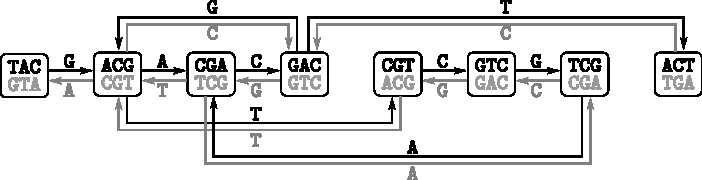
\includegraphics{dbg}
%	\end{center}
%	\caption{GDB de ordem $k=3$ da cadeia $S=\str{TACGACGTCGACT}$. Os nós são rotulados pelos 3-mers (em preto) e temos uma aresta dirigida $x_0x_1x_2\stackrel{y_2}\longrightarrow y_0y_1y_2$ sempre que $x_1x_2=y_0y_1$. Ocorre que, no sequenciamento de DNA, normalmente não sabemos se foi lida a sequência de uma fita ou da sua complementar, no sentido oposto. Portanto, o 4-mer $x_0x_1x_2x_3$ tanto pode representar a aresta $x_0x_1x_2\stackrel{x_3}\longrightarrow x_1x_2x_3$ como a aresta $x'_3x'_2x'_1\stackrel{x'_0}\longrightarrow x'_2x'_1x'_0$ ($x'j$ denota a base complementar de $x_j$). Por essa razão é comum identificar o nó ($k$-mer) com seu complemento reverso (em cinza) e considerar o grafo como bidirecional.}  \label{fig:dbg}
%\end{figure}


\clearpage
\section{Objetivos}

Os algoritmos escritos para responder uma sequência de queries de LCAs consistem em duas fases, que são o algoritmo de pré-processamento da árvore, com a finalidade de gerar uma estrutura de dados que facilite a resposta do LCA, e a query propriamente dita, que é um algoritmo escrito sobre essa nova estrutura de dados, cujo fim é responder objetivamente o LCA da query.

A abordagem proposta nesse trabalho busca modelar um pré-processamento econômico em termos de espaço e tempo, que permita que queries sejam respondidas num tempo razoavelmente curto.


\clearpage
\section{Metodologia}

O projeto será organizado nas atividades descritas abaixo e desenvolvidas conforme o cronograma a seguir.

\subsection{T0. Preparação da proposta}

Nesta fase inicial, aluno e orientador farão uma série de reuniões para definição do problema e escopo do projeto. O orientador apresentará a bibliografia básica sobre o tema e os possíveis pontos a serem abordados, e ambos decidirão sobre aqueles a serem desenvolvidos com base no  interesse mútuo.

\subsection{T1. Revisão e acompanhamento bibliográfico}

Essa tarefa será executada de maneira mais acentuada no início do projeto. A atividade consiste num estudo dirigido centrado no  material bibliográfico mais diretamente relacionado às estruturas de dados e algoritmos a serem implementados no projeto. Ao final dessa fase inicial, espera-se que o aluno possa manter-se atualizado e aprofundar-se em pontos específicos de maneira mais autônoma.


\subsection{T2. Implementação das estruturas}

Esta tarefa corresponde ao principal componente de desenvolvimento do projeto. O aluno deverá, em interação com o orientador, estudar detalhadamente algoritmos e estruturas de dados relativos a árvores, LCA, sparse tables, entre outros, e desenvolver uma implementação de referência em nível de produção para os mesmos, em C++.


\subsection{T3. Realização dos Testes}

Nesta tarefa, o aluno deverá fazer uma análise experimental comparativa do desempenho do método proposto e implementado relativamente a outras alternativas públicas identificadas num levantamento inicial na tarefa T1. Pode ser necessário obter dados reais e produzir dados sintéticos que simulem uma situação limite de estresse para os métodos.


\subsection{T4. Redação e revisão da monografia}

A monografia produzida deverá conter:
(1)~uma breve revisão bibliográfica do estado da arte, fruto da tarefa T1, (2)~descrição detalhada dos seus desenvolvimentos, incluindo a análise teórica dos algoritmos e estruturas propostas em termos de tempo e espaço, (3)~uma análise crítica com base em resultados experimentais da tarefa T3, e (4)~uma discussão com conclusões gerais sobre o projeto.


\subsection{T5. Preparação da Apresentação}

Finalmente, o aluno preparará a apresentação da defesa do TG com o resumo dos desenvolvimentos e resultados obtidos.

\medskip

O aluno já possui alguma familiaridade com a área, portanto poderá por-se rapidamente em desenvolvimento. O acompanhamento será feito pessoalmente através de reuniões semanais. Todo material desenvolvido é compartilhado entre orientador e aluno através de um repositório privado na plataforma GitHub. 


\clearpage
\section{Cronograma de atividades}


\begin{center}
	\begin{tabular}{| l || c | c | c | c | c | c | c | c | c | c | c | c | c | c | c |  c | c | c | c | }
		\hline
		& \multicolumn{2}{| c |}{Mar} & \multicolumn{4}{| c |}{Abr} & \multicolumn{4}{| c |}{Mai} & \multicolumn{4}{| c |}{Jun} & \multicolumn{2}{| c |}{Jul} \\\hline\hline
		Preparação da proposta & \X & \X & & & & & & & & & & & & & & \\\hline 
		Revisão bibliográfica$^\dagger$ & \X & \X & \x & \x & \x & \x & \x & \x & & & & & & & & \\\hline 
		Implementação das estruturas & & & \X & \X & \X & \X & \X & \X & \X & \X & \X & & & & & \\\hline 
		Realização dos testes$^\ddagger$ & & & & \x & \x & \x & \x & \x & \x  & \X & \X & \X & & & & \\\hline 
		Redação e revisão da monografia & & & & & & & & & & & \X & \X & \X & \X & & \\\hline 
		Preparação da apresentação & & & & & & & & & & & & & & & \X & \X \\\hline 
\hline
	\end{tabular}
\begin{minipage}{0.6\linewidth}
\noindent($\dagger$) \X = levantamento inicial, \x= aprofundamento\newline
\noindent($\ddagger$) \X= experimentos formais , \x = testes \textit{ad hoc} unitários\newline
\end{minipage}

\end{center}


\clearpage
%\nocite{*}
\bibliographystyle{unsrt-etal}
\bibliography{proposta}
%\printbibliography

\clearpage
\section{Possíveis Avaliadores}

\begin{enumerate}
\item Profa. Katia  Guimarães
\item Prof. Pedro Manhães
\end{enumerate}


\clearpage
\section{Assinaturas}

\vfill
\begin{center}
	Recife, 04 de Abril de 2018

	\vspace{3cm}
	\rule{10cm}{.5pt}\\
	\textbf{Aluno:} Daniel Cândido Cauás\\

	\vspace{3cm}
	\rule{10cm}{.5pt}\\
	\textbf{Orientador:} Paulo Gustavo Soares da Fonseca\\
\end{center}
\vfill

\end{document}

